\documentclass{standalone}
\usepackage{tikz}
\usetikzlibrary{patterns, positioning}


\begin{document}
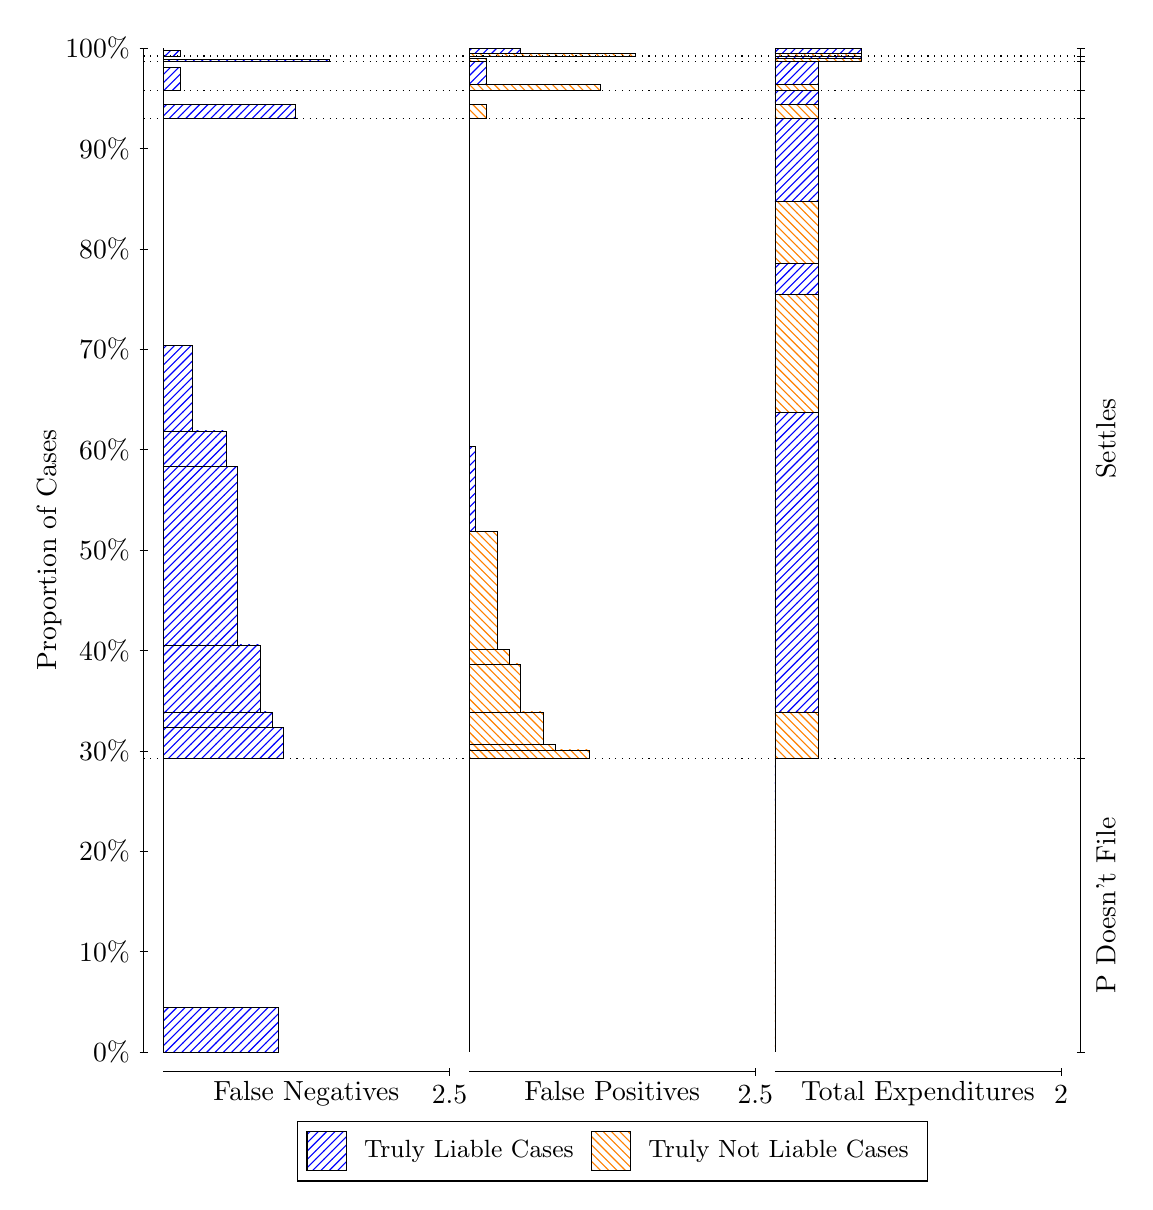
\begin{tikzpicture}
\draw[black, very thin] (1.5,1.75) -- (1.5,14.5);
\node[rotate=90, text=black, anchor=center] at (0.3, 8.125) {Proportion of Cases};
\draw[black, very thin] (1.45,1.75) -- (1.55,1.75);
\node[text=black, anchor=east] at (1.45, 1.75) {0\%};
\draw[black, very thin] (1.45,3.025) -- (1.55,3.025);
\node[text=black, anchor=east] at (1.45, 3.025) {10\%};
\draw[black, very thin] (1.45,4.3) -- (1.55,4.3);
\node[text=black, anchor=east] at (1.45, 4.3) {20\%};
\draw[black, very thin] (1.45,5.575) -- (1.55,5.575);
\node[text=black, anchor=east] at (1.45, 5.575) {30\%};
\draw[black, very thin] (1.45,6.85) -- (1.55,6.85);
\node[text=black, anchor=east] at (1.45, 6.85) {40\%};
\draw[black, very thin] (1.45,8.125) -- (1.55,8.125);
\node[text=black, anchor=east] at (1.45, 8.125) {50\%};
\draw[black, very thin] (1.45,9.4) -- (1.55,9.4);
\node[text=black, anchor=east] at (1.45, 9.4) {60\%};
\draw[black, very thin] (1.45,10.675) -- (1.55,10.675);
\node[text=black, anchor=east] at (1.45, 10.675) {70\%};
\draw[black, very thin] (1.45,11.95) -- (1.55,11.95);
\node[text=black, anchor=east] at (1.45, 11.95) {80\%};
\draw[black, very thin] (1.45,13.225) -- (1.55,13.225);
\node[text=black, anchor=east] at (1.45, 13.225) {90\%};
\draw[black, very thin] (1.45,14.5) -- (1.55,14.5);
\node[text=black, anchor=east] at (1.45, 14.5) {100\%};

\draw[black, very thin] (13.4,1.75) -- (13.4,14.5);
\draw[black, very thin] (13.35,1.75) -- (13.45,1.75);
\node[anchor=west] at (13.35, 1.75) {};
\draw[black, very thin] (13.35,5.4764) -- (13.45,5.4764);
\node[anchor=west] at (13.35, 5.4764) {};
\draw[black, very thin] (13.35,13.606) -- (13.45,13.606);
\node[anchor=west] at (13.35, 13.606) {};
\draw[black, very thin] (13.35,13.963) -- (13.45,13.963);
\node[anchor=west] at (13.35, 13.963) {};
\draw[black, very thin] (13.35,14.329) -- (13.45,14.329);
\node[anchor=west] at (13.35, 14.329) {};
\draw[black, very thin] (13.35,14.399) -- (13.45,14.399);
\node[anchor=west] at (13.35, 14.399) {};
\draw[black, very thin] (13.35,14.5) -- (13.45,14.5);
\node[anchor=west] at (13.35, 14.5) {};

\draw[black, very thin, pattern color=blue, pattern=north east lines] (1.75,1.75) rectangle (3.2033,2.312);
\draw[black, very thin, pattern color=orange, pattern=north west lines] (1.75,2.312) rectangle (1.75,5.4764);
\draw[black, very thin, pattern color=blue, pattern=north east lines] (1.75,5.4764) rectangle (3.276,5.87);
\draw[black, very thin, pattern color=blue, pattern=north east lines] (1.75,5.87) rectangle (3.1307,6.0699);
\draw[black, very thin, pattern color=blue, pattern=north east lines] (1.75,6.0699) rectangle (2.9853,6.9196);
\draw[black, very thin, pattern color=blue, pattern=north east lines] (1.75,6.9196) rectangle (2.6947,9.1903);
\draw[black, very thin, pattern color=blue, pattern=north east lines] (1.75,9.1903) rectangle (2.5493,9.637);
\draw[black, very thin, pattern color=blue, pattern=north east lines] (1.75,9.637) rectangle (2.1133,10.722);
\draw[black, very thin, pattern color=orange, pattern=north west lines] (1.75,10.722) rectangle (1.75,13.606);
\draw[black, very thin, pattern color=blue, pattern=north east lines] (1.75,13.606) rectangle (3.4213,13.781);
\draw[black, very thin, pattern color=orange, pattern=north west lines] (1.75,13.781) rectangle (1.75,13.963);
\draw[black, very thin, pattern color=blue, pattern=north east lines] (1.75,13.963) rectangle (1.968,14.255);
\draw[black, very thin, pattern color=orange, pattern=north west lines] (1.75,14.255) rectangle (1.75,14.329);
\draw[black, very thin, pattern color=blue, pattern=north east lines] (1.75,14.329) rectangle (3.8573,14.358);
\draw[black, very thin, pattern color=orange, pattern=north west lines] (1.75,14.358) rectangle (1.75,14.399);
\draw[black, very thin, pattern color=blue, pattern=north east lines] (1.75,14.399) rectangle (1.968,14.471);
\draw[black, very thin, pattern color=orange, pattern=north west lines] (1.75,14.471) rectangle (1.75,14.5);
\draw[black, very thin, pattern color=orange, pattern=north west lines] (5.6333,1.75) rectangle (5.6333,4.9144);
\draw[black, very thin, pattern color=blue, pattern=north east lines] (5.6333,4.9144) rectangle (5.6333,5.4764);
\draw[black, very thin, pattern color=orange, pattern=north west lines] (5.6333,5.4764) rectangle (7.1593,5.5858);
\draw[black, very thin, pattern color=orange, pattern=north west lines] (5.6333,5.5858) rectangle (6.7233,5.6548);
\draw[black, very thin, pattern color=orange, pattern=north west lines] (5.6333,5.6548) rectangle (6.578,6.0705);
\draw[black, very thin, pattern color=orange, pattern=north west lines] (5.6333,6.0705) rectangle (6.2873,6.6788);
\draw[black, very thin, pattern color=orange, pattern=north west lines] (5.6333,6.6788) rectangle (6.142,6.8638);
\draw[black, very thin, pattern color=orange, pattern=north west lines] (5.6333,6.8638) rectangle (5.9967,8.3608);
\draw[black, very thin, pattern color=blue, pattern=north east lines] (5.6333,8.3608) rectangle (5.706,9.4453);
\draw[black, very thin, pattern color=blue, pattern=north east lines] (5.6333,9.4453) rectangle (5.6333,13.606);
\draw[black, very thin, pattern color=orange, pattern=north west lines] (5.6333,13.606) rectangle (5.8513,13.788);
\draw[black, very thin, pattern color=blue, pattern=north east lines] (5.6333,13.788) rectangle (5.6333,13.963);
\draw[black, very thin, pattern color=orange, pattern=north west lines] (5.6333,13.963) rectangle (7.3047,14.037);
\draw[black, very thin, pattern color=blue, pattern=north east lines] (5.6333,14.037) rectangle (5.8513,14.329);
\draw[black, very thin, pattern color=orange, pattern=north west lines] (5.6333,14.329) rectangle (5.8513,14.371);
\draw[black, very thin, pattern color=blue, pattern=north east lines] (5.6333,14.371) rectangle (5.6333,14.399);
\draw[black, very thin, pattern color=orange, pattern=north west lines] (5.6333,14.399) rectangle (7.7407,14.428);
\draw[black, very thin, pattern color=blue, pattern=north east lines] (5.6333,14.428) rectangle (6.2873,14.5);
\draw[black, very thin, pattern color=orange, pattern=north west lines] (9.5167,1.75) rectangle (9.5167,4.9144);
\draw[black, very thin, pattern color=blue, pattern=north east lines] (9.5167,4.9144) rectangle (9.5167,5.4764);
\draw[black, very thin, pattern color=orange, pattern=north west lines] (9.5167,5.4764) rectangle (10.062,6.0705);
\draw[black, very thin, pattern color=blue, pattern=north east lines] (9.5167,6.0705) rectangle (10.062,9.8724);
\draw[black, very thin, pattern color=orange, pattern=north west lines] (9.5167,9.8724) rectangle (10.062,11.369);
\draw[black, very thin, pattern color=blue, pattern=north east lines] (9.5167,11.369) rectangle (10.062,11.763);
\draw[black, very thin, pattern color=orange, pattern=north west lines] (9.5167,11.763) rectangle (10.062,12.556);
\draw[black, very thin, pattern color=blue, pattern=north east lines] (9.5167,12.556) rectangle (10.062,13.606);
\draw[black, very thin, pattern color=orange, pattern=north west lines] (9.5167,13.606) rectangle (10.062,13.788);
\draw[black, very thin, pattern color=blue, pattern=north east lines] (9.5167,13.788) rectangle (10.062,13.963);
\draw[black, very thin, pattern color=orange, pattern=north west lines] (9.5167,13.963) rectangle (10.062,14.037);
\draw[black, very thin, pattern color=blue, pattern=north east lines] (9.5167,14.037) rectangle (10.062,14.329);
\draw[black, very thin, pattern color=orange, pattern=north west lines] (9.5167,14.329) rectangle (10.607,14.371);
\draw[black, very thin, pattern color=blue, pattern=north east lines] (9.5167,14.371) rectangle (10.607,14.399);
\draw[black, very thin, pattern color=orange, pattern=north west lines] (9.5167,14.399) rectangle (10.607,14.428);
\draw[black, very thin, pattern color=blue, pattern=north east lines] (9.5167,14.428) rectangle (10.607,14.5);
\draw[black, dotted] (1.5,5.4764) -- (13.4,5.4764);
\draw[black, dotted] (1.5,13.606) -- (13.4,13.606);
\draw[black, dotted] (1.5,13.963) -- (13.4,13.963);
\draw[black, dotted] (1.5,14.329) -- (13.4,14.329);
\draw[black, dotted] (1.5,14.399) -- (13.4,14.399);
\draw[black, very thin] (1.75,1.5) -- (5.3833,1.5);
\node[text=black, anchor=north] at (3.5667, 1.5) {False Negatives};
\draw[black, very thin] (5.3833,1.45) -- (5.3833,1.55);
\node[text=black, anchor=north] at (5.3833, 1.45) {2.5};

\draw[black, very thin] (5.6333,1.5) -- (9.2667,1.5);
\node[text=black, anchor=north] at (7.45, 1.5) {False Positives};
\draw[black, very thin] (9.2667,1.45) -- (9.2667,1.55);
\node[text=black, anchor=north] at (9.2667, 1.45) {2.5};

\draw[black, very thin] (9.5167,1.5) -- (13.15,1.5);
\node[text=black, anchor=north] at (11.333, 1.5) {Total Expenditures};
\draw[black, very thin] (13.15,1.45) -- (13.15,1.55);
\node[text=black, anchor=north] at (13.15, 1.45) {2};

\node[text=black, centered, rotate=90] at (13.72, 3.6132) {P Doesn't File};
\node[text=black, centered, rotate=90] at (13.72, 9.5412) {Settles};





\draw (7.449999999999999,1.5) node[draw=none] (baseCoordinate) {};
\begin{scope}[align=center]
        \matrix[scale=0.5, draw=black, below=0.5cm of baseCoordinate, nodes={draw}, column sep=0.1cm]{
            \node[rectangle, draw, minimum width=0.5cm, minimum height=0.5cm, pattern color=blue, pattern=north east lines] {}; &
            \node[draw=none, font=\small, text=black] (B) {Truly Liable Cases}; &
            \node[rectangle, draw, minimum width=0.5cm, minimum height=0.5cm, pattern color=orange, pattern=north west lines] {}; &
            \node[draw=none, font=\small, text=black] (B) {Truly Not Liable Cases}; \\
            };
\end{scope}

\end{tikzpicture}
\end{document}